\documentclass{beamer}
\mode<presentation>
\usepackage{amsmath,amssymb,mathtools}
\usepackage{textcomp}
\usepackage{gensymb}
\usepackage{adjustbox}
\usepackage{subcaption}
\usepackage{enumitem}
\usepackage{multicol}
\usepackage{listings}
\usepackage{url}
\usepackage{graphicx} % <-- needed for images
\def\UrlBreaks{\do\/\do-}

\usetheme{Boadilla}
\usecolortheme{lily}
\setbeamertemplate{footline}{
  \leavevmode%
  \hbox{%
  \begin{beamercolorbox}[wd=\paperwidth,ht=2ex,dp=1ex,right]{author in head/foot}%
    \insertframenumber{} / \inserttotalframenumber\hspace*{2ex}
  \end{beamercolorbox}}%
  \vskip0pt%
}
\setbeamertemplate{navigation symbols}{}

\lstset{
  frame=single,
  breaklines=true,
  columns=fullflexible,
  basicstyle=\ttfamily\tiny   % tiny font so code fits
}

\numberwithin{equation}{section}

% ---- your macros ----
\providecommand{\nCr}[2]{\,^{#1}C_{#2}}
\providecommand{\nPr}[2]{\,^{#1}P_{#2}}
\providecommand{\mbf}{\mathbf}
\providecommand{\pr}[1]{\ensuremath{\Pr\left(#1\right)}}
\providecommand{\qfunc}[1]{\ensuremath{Q\left(#1\right)}}
\providecommand{\sbrak}[1]{\ensuremath{{}\left[#1\right]}}
\providecommand{\lsbrak}[1]{\ensuremath{{}\left[#1\right.}}
\providecommand{\rsbrak}[1]{\ensuremath{\left.#1\right]}}
\providecommand{\brak}[1]{\ensuremath{\left(#1\right)}}
\providecommand{\lbrak}[1]{\ensuremath{\left(#1\right.}}
\providecommand{\rbrak}[1]{\ensuremath{\left.#1\right)}}
\providecommand{\cbrak}[1]{\ensuremath{\left\{#1\right\}}}
\providecommand{\lcbrak}[1]{\ensuremath{\left\{#1\right.}}
\providecommand{\rcbrak}[1]{\ensuremath{\left.#1\right\}}}
\theoremstyle{remark}
\newtheorem{rem}{Remark}
\newcommand{\sgn}{\mathop{\mathrm{sgn}}}
\providecommand{\abs}[1]{\left\vert#1\right\vert}
\providecommand{\res}[1]{\Res\displaylimits_{#1}}
\providecommand{\norm}[1]{\lVert#1\rVert}
\providecommand{\mtx}[1]{\mathbf{#1}}
\providecommand{\mean}[1]{E\left[ #1 \right]}
\providecommand{\fourier}{\overset{\mathcal{F}}{ \rightleftharpoons}}
\providecommand{\system}{\overset{\mathcal{H}}{ \longleftrightarrow}}
\providecommand{\dec}[2]{\ensuremath{\overset{#1}{\underset{#2}{\gtrless}}}}
\newcommand{\myvec}[1]{\ensuremath{\begin{pmatrix}#1\end{pmatrix}}}
\let\vec\mathbf
% ---------------------

\title{Matgeo Presentation - Problem 2.5.19}
\author{ee25btech11056 - Suraj.N}

\begin{document}

\begin{frame}
  \titlepage
\end{frame}

% Problem Statement
\begin{frame}{Problem Statement}

  \textbf{Question} : Find the value of $p$ for which the lines $\dfrac{1-x}{3}=\dfrac{2y-14}{2p}=\dfrac{z-3}{2}$ and $\dfrac{1-x}{3p}=\dfrac{y-5}{1}=\dfrac{6-z}{5}$ are perpendicular.

\begin{table}[h!]
  \centering
  

  \caption*{Table : Lines}
  \label{2.5.19}
\end{table}

\end{frame}

\begin{frame}{Solution}

  These lines can also be written in the vector form $\vec{x}=\vec{h}+k\vec{m}$ .

\begin{align*}
  \text{Line A: }\;\; \vec{x}=\myvec{1\\7\\3}+k_1\myvec{-3\\p\\2} \\
  \text{Line B: }\;\; \vec{x}=\myvec{1\\5\\6}+k_2\myvec{-3p\\1\\-5}
\end{align*}

Hence, the direction vectors are
\begin{align*}
  \vec{m_1}=\myvec{-3\\ p\\ 2}, \qquad
  \vec{m_2}=\myvec{-3p\\ 1\\ -5}.
\end{align*}

\end{frame}

\begin{frame}

  For the lines to be perpendicular, we require $\vec{m_1^\top} \vec{m_2}=0$.

\begin{align*}
  \vec{m_1^\top} \vec{m_2}
&= \myvec{-3 & p & 2}\myvec{-3p\\ 1\\ -5} \\
&= (-3)(-3p) + p(1) + 2(-5) \\
&= 9p + p - 10 \\
&= 10p - 10.
\end{align*}

Thus,
\begin{align*}
10p - 10 = 0 \;\Rightarrow\; p=1.
\end{align*}

\textbf{Final answer:} $p=1$.

\end{frame}

\begin{frame}{Plot}

\begin{figure}[h!]
  \centering
  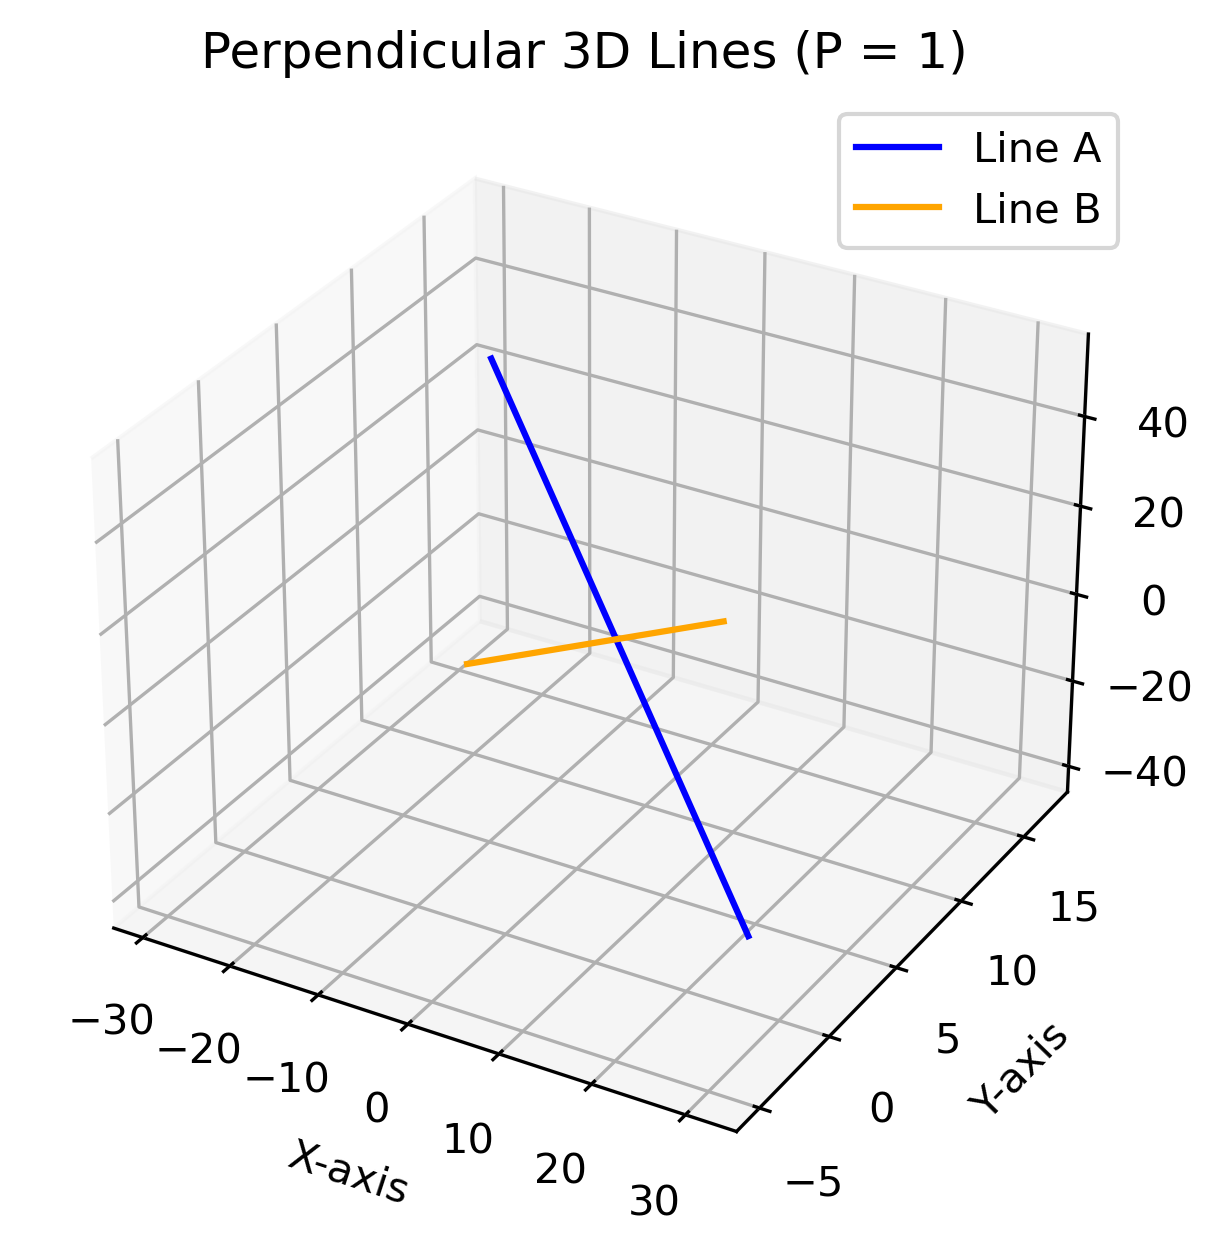
\includegraphics[width=0.5\columnwidth]{figs/perpendicular_lines.png} 
   \caption*{Fig : Lines A and B}
  \label{Fig1}
\end{figure}

\end{frame}

\section*{Appendix: Code}

% C program
\begin{frame}[fragile]{C Code: points.c}
\begin{lstlisting}[language=C]

#include <math.h>
#include <stdio.h>

// Return the dot product instead of p
double product(double p) {
  double dot = 0;
  double a[3] = {-3, p, 2};
  double b[3] = {-3 * p, 1, -5};

  for (int i = 0; i < 3; i++) {
    dot += a[i] * b[i];
  }
  return dot; // return dot product
}
\end{lstlisting}
\end{frame}

% Python calling C
\begin{frame}[fragile]{Python: call\_c.py}
\begin{lstlisting}[language=Python]

import ctypes
import sys
import numpy as np
import matplotlib.pyplot as plt

# Load shared library
lib = ctypes.CDLL("./points.so")
lib.product.restype = ctypes.c_double
lib.product.argtypes = [ctypes.c_double]

solution_p = None
for p in range(-10, 11):
    dot = lib.product(ctypes.c_double(p))
    if abs(dot) < 1e-6:   # check near zero
        solution_p = p
        print(f"Solution found: p = {p}")
        break

if solution_p is None:
    print("No solution found")
    sys.exit(0)

p = solution_p

# Parametric equations
t = np.linspace(-10, 10, 100)
x1 = 1 - 3*t
y1 = 7 + p*t
z1 = 3 + 2*t

\end{lstlisting}
\end{frame}

\begin{frame}[fragile]{Python: call\_c.py}
\begin{lstlisting}[language=Python]

s = np.linspace(-10, 10, 100)
x2 = 1 - 3*p*s
y2 = 5 + s
z2 = 6 - 5*s

# Plotting
fig = plt.figure()
ax = fig.add_subplot(111, projection='3d')

ax.plot(x1, y1, z1, label="Line A", color="blue")
ax.plot(x2, y2, z2, label="Line B", color="orange")

ax.set_title("Perpendicular 3D Lines (P = 1)")
ax.set_xlabel("X-axis")
ax.set_ylabel("Y-axis")
ax.set_zlabel("Z-axis")
ax.legend()

# Save the figure
plt.savefig("perpendicular_lines.png", dpi=300, bbox_inches="tight")

# Show the plot
plt.show()

\end{lstlisting}
\end{frame}

% Python plotting
\begin{frame}[fragile]{Python: plot.py}
\begin{lstlisting}[language=Python]

import numpy as np
import matplotlib.pyplot as plt

# Directly use the analytical solution
p = 1

# Parametric equations for Line 1 and Line 2
t = np.linspace(-10, 10, 200)
x1 = 1 - 3*t
y1 = 7 + p*t
z1 = 3 + 2*t

s = np.linspace(-10, 10, 200)
x2 = 1 - 3*p*s
y2 = 5 + s
z2 = 6 - 5*s

# Plotting
fig = plt.figure(figsize=(8,6))
ax = fig.add_subplot(111, projection='3d')

ax.plot(x1, y1, z1, label="Line A", color="blue", linewidth=2)
ax.plot(x2, y2, z2, label="Line B", color="orange", linewidth=2)

ax.set_title("Perpendicular 3D Lines (p = 1)")
ax.set_xlabel("X-axis")
ax.set_ylabel("Y-axis")
ax.set_zlabel("Z-axis")
ax.legend()

# Save the figure
plt.savefig("perpendicular_lines.png", dpi=300, bbox_inches="tight")

# Show the plot
plt.show()

\end{lstlisting}
\end{frame}

\end{document}
